% Primary source: https://arxiv.org/abs/1704.01212
\documentclass[tikz,border=5pt]{standalone}
\usepackage[T1]{fontenc}
\usepackage{lmodern,amsmath,amssymb}
\usetikzlibrary{arrows.meta,calc,positioning,fit,backgrounds,shapes.geometric,matrix,decorations.pathreplacing,patterns}
\definecolor{ink}{gray}{0.08}
\definecolor{wash}{gray}{0.965}
\definecolor{soft}{gray}{0.45}
\tikzset{box/.style={draw=ink,line width=.65pt,fill=white,align=center,inner sep=4pt,outer sep=0pt,font=\small},flow/.style={draw=ink,line width=.65pt,-{Latex[length=1.8mm,width=1.3mm]},rounded corners=2pt},annotation/.style={font=\scriptsize,text=soft,align=center},groupbox/.style={draw=soft,dashed,line width=.45pt,fill=wash}}
\begin{document}
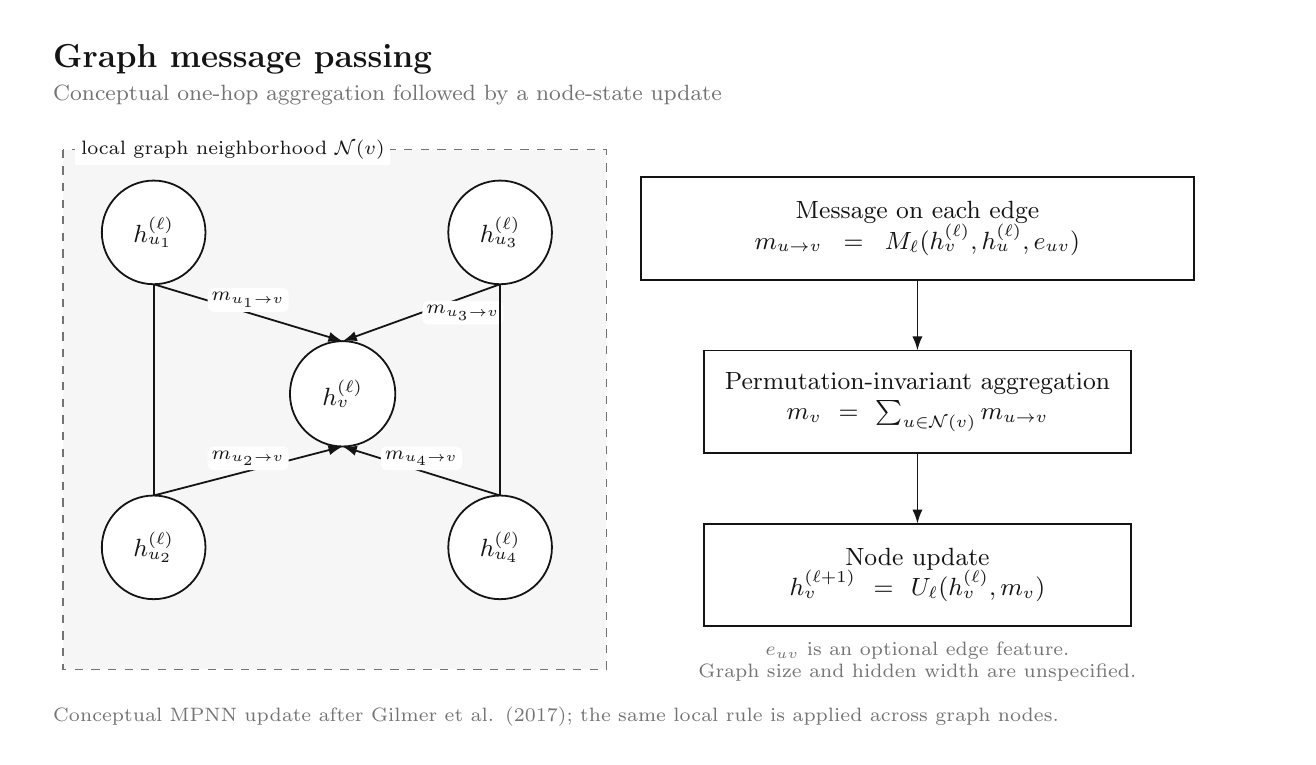
\begin{tikzpicture}[x=1cm,y=-1cm,font=\rmfamily,text=ink]

\path[use as bounding box] (0,0) rectangle (16,9);
\node[anchor=west,font=\large\bfseries] at (.2,.4) {Graph message passing};
\node[anchor=west,font=\footnotesize,text=soft] at (.2,.85) {Conceptual one-hop aggregation followed by a node-state update};
\begin{pgfonlayer}{background}
\draw[groupbox] (0.45,1.55) rectangle (7.3500000000000005,8.15);
\node[anchor=west,font=\scriptsize,fill=white,inner sep=2pt] at (0.6,1.55) {local graph neighborhood $\mathcal{N}(v)$};
\end{pgfonlayer}
\node[box,circle,minimum width=1.15cm,minimum height=1.15cm,text width=0.8999999999999999cm] (v) at (4.0,4.65) {$h_v^{(\ell)}$};
\node[box,circle,minimum width=1.1cm,minimum height=1.1cm,text width=0.8500000000000001cm] (u1) at (1.6,2.6) {$h_{u_1}^{(\ell)}$};
\node[box,circle,minimum width=1.1cm,minimum height=1.1cm,text width=0.8500000000000001cm] (u2) at (1.6,6.6) {$h_{u_2}^{(\ell)}$};
\node[box,circle,minimum width=1.1cm,minimum height=1.1cm,text width=0.8500000000000001cm] (u3) at (6.0,2.6) {$h_{u_3}^{(\ell)}$};
\node[box,circle,minimum width=1.1cm,minimum height=1.1cm,text width=0.8500000000000001cm] (u4) at (6.0,6.6) {$h_{u_4}^{(\ell)}$};
\node[box,minimum width=7.0cm,minimum height=1.3cm,text width=6.75cm] (message) at (11.3,2.55) {Message on each edge\\$m_{u\to v}=M_\ell(h_v^{(\ell)},h_u^{(\ell)},e_{uv})$};
\node[box,minimum width=5.4cm,minimum height=1.3cm,text width=5.15cm] (aggregate) at (11.3,4.75) {Permutation-invariant aggregation\\$m_v=\sum_{u\in\mathcal{N}(v)}m_{u\to v}$};
\node[box,minimum width=5.4cm,minimum height=1.3cm,text width=5.15cm] (update) at (11.3,6.95) {Node update\\$h_v^{(\ell+1)}=U_\ell(h_v^{(\ell)},m_v)$};
\begin{pgfonlayer}{background}
\draw[flow] (u1.south) -- (v.north) node[midway,above,fill=white,inner sep=1.5pt,font=\scriptsize] {$m_{u_1\to v}$};
\draw[flow] (u2.north) -- (v.south) node[midway,above,fill=white,inner sep=1.5pt,font=\scriptsize] {$m_{u_2\to v}$};
\draw[flow] (u3.south) -- (v.north) node[midway,right,fill=white,inner sep=1.5pt,font=\scriptsize] {$m_{u_3\to v}$};
\draw[flow] (u4.north) -- (v.south) node[midway,above,fill=white,inner sep=1.5pt,font=\scriptsize] {$m_{u_4\to v}$};
\draw[flow,-] (u1.south) -- (u2.north);
\draw[flow,-] (u3.south) -- (u4.north);
\draw[flow] (message.south) -- (aggregate.north);
\draw[flow] (aggregate.south) -- (update.north);
\end{pgfonlayer}
\node[annotation,text width=7.0cm] at (11.3,8.05) {$e_{uv}$ is an optional edge feature.\\Graph size and hidden width are unspecified.};
\node[anchor=west,align=left,font=\scriptsize,text=soft,text width=15.6cm] at (.2,8.75) {Conceptual MPNN update after Gilmer et al. (2017); the same local rule is applied across graph nodes.};
\end{tikzpicture}
\end{document}
